%----------------------------------------------------------------------------------------
%	PACKAGES AND OTHER DOCUMENT CONFIGURATIONS
%----------------------------------------------------------------------------------------
\documentclass[paper=a4, fontsize=11pt]{scrartcl} % A4 paper and 11pt font size

\usepackage[T1]{fontenc} % Use 8-bit encoding that has 256 glyphs
\usepackage{fourier} % Use the Adobe Utopia font for the document - comment this line to return to the LaTeX default
\usepackage[english]{babel} % English language/hyphenation
\usepackage{amsmath,amsfonts,amsthm,amssymb} % Math packages
\usepackage{mathrsfs}
\usepackage{algorithm, algorithmic}
\renewcommand{\algorithmicrequire}{\textbf{Input:}} %Use Input in the format of Algorithm  
\renewcommand{\algorithmicensure}{\textbf{Output:}} %UseOutput in the format of Algorithm  
\usepackage{listings}
\lstset{language=Matlab}
\usepackage{enumerate}
\usepackage{graphicx}

\usepackage{lipsum} % Used for inserting dummy 'Lorem ipsum' text into the template
\usepackage{sectsty} % Allows customizing section commands
\allsectionsfont{\centering \normalfont\scshape} % Make all sections centered, the default font and small caps
\usepackage{fancyhdr} % Custom headers and footers
\pagestyle{fancyplain} % Makes all pages in the document conform to the custom headers and footers
\fancyhead{} % No page header - if you want one, create it in the same way as the footers below
\fancyfoot[L]{} % Empty left footer
\fancyfoot[C]{} % Empty center footer
\fancyfoot[R]{\thepage} % Page numbering for right footer
\renewcommand{\headrulewidth}{0pt} % Remove header underlines
\renewcommand{\footrulewidth}{0pt} % Remove footer underlines
\setlength{\headheight}{13.6pt} % Customize the height of the header

\numberwithin{equation}{section} % Number equations within sections (i.e. 1.1, 1.2, 2.1, 2.2 instead of 1, 2, 3, 4)
\numberwithin{figure}{section} % Number figures within sections (i.e. 1.1, 1.2, 2.1, 2.2 instead of 1, 2, 3, 4)
\numberwithin{table}{section} % Number tables within sections (i.e. 1.1, 1.2, 2.1, 2.2 instead of 1, 2, 3, 4)

\setlength\parindent{0pt} % Removes all indentation from paragraphs - comment this line for an assignment with lots of text

%----------------------------------------------------------------------------------------
%	TITLE SECTION
%----------------------------------------------------------------------------------------
\newcommand{\horrule}[1]{\rule{\linewidth}{#1}} % Create horizontal rule command with 1 argument of height

\title{	
\normalfont \normalsize 
\textsc{Shanghai Jiao Tong University, UM-SJTU JOINT INSTITUTE} \\ [25pt] % Your university, school and/or department name(s)
\horrule{0.5pt} \\[0.4cm] % Thin top horizontal rule
\huge Introduction to Numerical Analysis \\ Project2 \\ % The assignment title
\horrule{2pt} \\[0.5cm] % Thick bottom horizontal rule
}

\author{Yu Cang \\ 018370210001} % Your name

\date{\normalsize \today} % Today's date or a custom date

\begin{document}

\maketitle % Print the title

\section{Task 1}
	Note the symmetry of $x_1$, for any solution $(a, b)$, $(-a, b)$ is also valid.\\
	If no special claim, the norm function for a vector is taken as the 2-norm.
	\begin{enumerate}[(a)]
		\item
			For fixed-point iteration, the iteration function $G$ is taken as
			\begin{equation}
				G \triangleq
				\begin{bmatrix}
					\sqrt{x_2}\\
					\sqrt{1-x_1^2}
				\end{bmatrix}
				=
				\begin{bmatrix}
					x_1\\
					x_2\\
				\end{bmatrix}
				=x
			\end{equation}
			The iteration converges to $(0.7862, 0.6180)$ with intial guess $x_{init} = [\frac{1}{\sqrt{2}}, \frac{1}{\sqrt{2}}]^T$ and tolerance set to $10^{-10}$. 
		\item 
			The newton iteration is implemented as mentioned in the project sheet, each time the linear system
			\begin{equation}
				J_F(x_k) w_k = y_k
			\end{equation}
			is solved with the built-in function 'linsolve' inside matlab.\\
			The iteration converges to $(0.7862, 0.6180)$ with intial guess $x_{init} = [\frac{1}{\sqrt{2}}, \frac{1}{\sqrt{2}}]^T$ and tolerance set to $10^{-10}$. 
		\item
			The input of the Broyden's method is a little bit different from that in newton or fixed-point. The initial Jacobi matrix should be provided, denoted as $A_0$. In my implementation, it is given as
			\begin{equation}
				A_0 = J_F(x_0)
			\end{equation}
			An extra calculation on $x_1$ should be done before the iteration loop as the iteration process requires both $x_0$ and $x_1$. It is approximated through newton's method in my implementation as
			\begin{equation}
				x_1 \approxeq x_0 - A_0^{-1}F(x_0)
			\end{equation}
			After all the preparation work, the iteration loop can be carried out as mentioned in the project sheet, and the key part is the application of Sherman-Morrison's formula to calculated the inverse of $A_k$ iteratively as
			\begin{equation}
				A_k^{-1} = A_{k-1}^{-1} + \frac{(s_k^T A_{k-1}^{-1} y_k)s_k^T A_{k-1}^{-1}}{s_k^T A_{k-1}^{-1} y_k}
			\end{equation}
			where $s_k = x_k - x_{k-1}$ and $y_k = F(x_k) - F(x_{k-1})$. And the iteration of $x_k$ is given as
			\begin{equation}
				x_{k+1} = x_k - A_k^{-1}F(x_k)
			\end{equation}
			The iteration converges to $(0.7862, 0.6180)$ with intial guess $x_{init} = [\frac{1}{\sqrt{2}}, \frac{1}{\sqrt{2}}]^T$ and tolerance set to $10^{-10}$. 
		\item 
			With numerical tests, newton's method out-performs the other two in terms of time cost.
		
	\end{enumerate}

\section{Task 2}
	With trival inequality analysis, the exact solution is given as $x=[0.5, 0, -\frac{\pi}{6}]$, which can be used for varification.
	\subsection{Solve directly}
		Applying the fixed-point iteration, newton's method and the broyden's method to this non-linear system respectively, ...(TODO)
	\subsection{Downhill simplex algorithm}
	In general, the initial value for such a non-linear system is hard to know, even the range for each component is hard to estimate. In this case, the downhill simplex method can be applied to produce a fine inital guess for further calculation like newton or quasi-newton.
	\subsection{Solve with initialization}
	
	Numerical experiments were done to identify the difference in terms of time cost. 
	
	\begin{center}
		\begin{tabular}{ccc}
			\hline
			\quad       & Without initialization & With initialization\\
			\hline
			fixed-point & $4.033 ms$             & $3.970 ms$\\
			neweon      & $4.661 ms$             & $0.679 ms$\\
			broyden     & $4.447 ms$             & $0.799 ms$\\
			\hline
		\end{tabular}
	\end{center}
	
	It can be observed from the table that the downhill simplex initialization process does help a lot to reduce time cost for further newton or broyden calculation as it provide a better initial guess. \\
	However, the time cost is almost equivalent for the fixed-point iteration, which indicates that it does not benefit from the downhill simplex initialization. 

\section{Task 3}
	\begin{enumerate}[(a)]
		\item 
			Denote $y_1(t) \triangleq n(t)$, $y_2(t) \triangleq x(t)$ and
			\begin{equation}
				\Phi \triangleq
				\begin{bmatrix}
					\dot{y_1}\\
					 \dot{y_2}	
				\end{bmatrix}
				=
				\begin{bmatrix}
					\gamma - \alpha y_2^2 y_1\\
					\alpha y_2^2 y_1 - \frac{y_1}{1+y_1}
				\end{bmatrix}
			\end{equation}
			Then, the synthetic data for $n$ and $x$ can be calculated iteratively. To make it more accurate, the Runge-Kutta 4-stage method was adopted. The matlab built-in function 'ode45' was used in my implementation. \\
			Plot of $n(t)$ and $x(t)$ were generated as follows
			\begin{figure}[htbp]\centering
				\begin{minipage}{7.5cm}
					\centering
					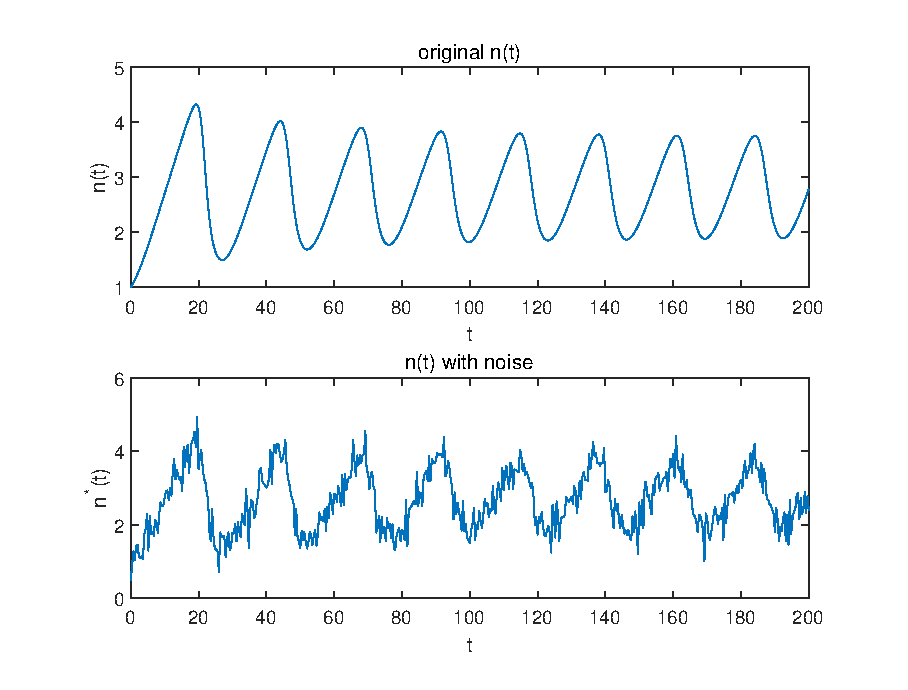
\includegraphics[height=7cm,width=7cm]{../pic/n_and_ns.eps}
				\end{minipage}%
				\begin{minipage}{7.5cm}
					\centering
					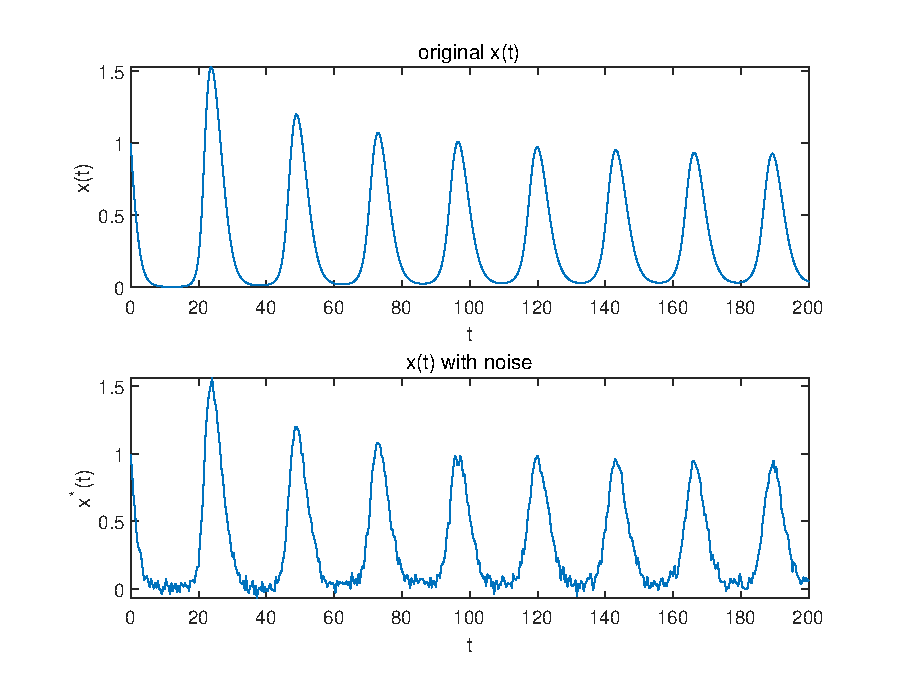
\includegraphics[height=7cm,width=7cm]{../pic/x_and_xs.eps}
				\end{minipage}
			\end{figure}
		
			Plot of $n(t)$ and $x(t)$ with noise were also generated here to make a clear comparsion.
		\item 
			At each point (except the two boundary points), the 1st-order derivative of $n(t)$ and $x(t)$ can be approximated using central difference as
			\begin{equation}
				\dot{n_k} = \frac{n_{k+1}-n_{k-1}}{2 \Delta t} \label{si_eq1}
			\end{equation}
			\begin{equation}
				\dot{x_k} = \frac{x_{k+1}-x_{k-1}}{2 \Delta t} \label{si_eq2}
			\end{equation}
			Thus a pair of $\alpha$ and $\gamma$ can be solved at each point as
			\begin{equation}
				\alpha_k = \frac{\dot{x_k} + \frac{x_k}{1+x_k}}{n_k^2x_k}
			\end{equation}
			\begin{equation}
				\gamma_k = \dot{x_k} + \dot{n_k} + \frac{x_k}{1+x_k}
			\end{equation}
			for $k=2,3,...,N-1$.\\
			Finally, the estimated $\alpha$ and $\gamma$ can be calculated as
			\begin{equation}
				\hat{\alpha} = \frac{\sum_{k=2}^{N-1}\alpha_k}{N-2}
			\end{equation}
			\begin{equation}
				\hat{\gamma} = \frac{\sum_{k=2}^{N-1}\gamma_k}{N-2}
			\end{equation}
			Numerical experiment shows that $\hat{\alpha} = 0.099824$ and $\hat{\gamma} = 0.199699$, which implies that $\hat{\alpha}$ and $\hat{\gamma}$ agree well with $\alpha$ and $\gamma$.
		\item 
			The noise is generated with the built-in function 'normrnd' of matlab in my code, plots are given in part(a). 

		\item 
			Considering the mathmatical expect of $Eq(\ref{si_eq1})$ and $Eq(\ref{si_eq2})$ as
			\begin{equation}
				\begin{aligned}
					E(\dot{n}) & = \gamma - \alpha E(n^2 x)\\
					E(\dot{x}) & = \alpha E(n^2 x) - E(\frac{x}{1+x})
				\end{aligned}
			\end{equation}
			Then $\alpha$ and $\gamma$ can be resolved as
			\begin{equation}
				\begin{aligned}
					\hat{\alpha} & = \frac{E(\dot{x}) + E(\frac{x}{1+x})}{E(n^2 x)}\\
					\hat{\gamma} & = E(\dot{x}) + E(\dot{n}) + E(\frac{x}{1+x})
				\end{aligned}
			\end{equation}
			But the signal we have is not clean, what we can obtain from the data are quantities with noise like $E(\dot{n^*})$, $E(\dot{x^*})$, $E({n^*}^2 x^*)$, and $E(\frac{x^*}{1+x^*})$. These clean quantities like $E(\dot{n})$, $E(\dot{x})$, $E(n^2 x)$, and $E(\frac{x}{1+x})$ should be approximated from these polluted quantities so that $\hat{\alpha}$ and $\hat{\gamma}$ can be resolved.\\
			As $\epsilon \sim N(0, 0.01)$ and $\nu \sim N(0, 0.001)$, then $E(\epsilon) = 0$, $E(\nu) = 0$ and $E(\epsilon^2) = 0.01$, $E(\nu^2)=0.001$.
			Since $n^* = n + \epsilon$ and $x^* = x + \nu$, then
			\begin{equation}
				\begin{aligned}
					E(n^*) & = E(n) + E(\epsilon) = E(n)\\
					E(x^*) & = E(x) + E(\nu) = E(x)
				\end{aligned}
			\end{equation}
			As $\epsilon$ and $\nu$ are independent, thus
			\begin{equation}
				\begin{aligned}
					E({n^*}^2 x^*) & = E(n^2 x + 2nx\epsilon + x\epsilon^2 + n^2\nu + 2n\epsilon\nu + \epsilon^2 \nu)\\
					               & = E(n^2 x) + E(x)E(\epsilon^2)
				\end{aligned}
			\end{equation}
			and
			\begin{equation}
				E(\frac{x^*}{1+x^*}) = E(\frac{x}{1+x^*}) \approxeq E(\frac{x}{1+x})
			\end{equation}
			For derivatives, similiar relation can be concluded as
			\begin{equation}
				\begin{aligned}
					E(\dot{n_k^*}) & = \frac{E(n_{k+1}^*) - E(n_{k-1}^*)}{2 \Delta t} = \frac{E(n_{k+1}) - E(n_{k-1})}{2 \Delta t} = E(\dot{n_k})\\
					E(\dot{x_k^*}) & = \frac{E(x_{k+1}^*) - E(x_{k-1}^*)}{2 \Delta t} = \frac{E(x_{k+1}) - E(x_{k-1})}{2 \Delta t} = E(\dot{x_k})
				\end{aligned}
			\end{equation}
			Hence these clean quantities can be approximated as
			\begin{equation}
				\begin{aligned}
					E(n) & = E(n^*)\\
					E(x) & = E(x^*)\\
					E(\dot{n}) & = E(\dot{n^*}) = \frac{\sum_{k=2}^{N-1}\dot{n_k^*}}{N-2}\\
					E(\dot{x}) & = E(\dot{x^*}) = \frac{\sum_{k=2}^{N-1}\dot{x_k^*}}{N-2}\\
					E(n^2 x) & = E({n^*}^2 x^*) - E(x)E(\epsilon^2)\\
					E(\frac{x}{1+x}) & = E(\frac{x^*}{1+x^*})
				\end{aligned}
			\end{equation}
			where the properties of the noise is utilized.\\
			In this way, $\hat{\alpha}$ and $\hat{\gamma}$ were resolved in numerical experiment as
			\begin{equation}
				\begin{aligned}
					\hat{\alpha} & = 0.102744\\
					\hat{\gamma} & = 0.201082
				\end{aligned}
			\end{equation}
			The result has been validated for about 20 times, although the noise is different at each time, as well as $\hat{\alpha}$ and $\hat{\gamma}$, but each time the result was quite stable.
		\item 
			If the properties of noise are not available, some approximations or assumptions can not be made finely.\\
			At first, a distinct attempt is to treat $n^*$ and $x^*$ like what we have done in part(b).
			\begin{equation}
				\hat{\alpha} = \frac{\sum_{k=2}^{N-1}\alpha_k^*}{N-2}
			\end{equation}
			\begin{equation}
				\hat{\gamma} = \frac{\sum_{k=2}^{N-1}\gamma_k^*}{N-2}
			\end{equation}
			In this way, the only difference is the input data sequence, as the input in part(b) is clean but here is polluted. \\
			Numerical experiments were done for 200 times to illustrate the initial guess(Fig\ref{coarse_ag}) and the variance(Fig\ref{err_ag}) of $\hat{\alpha}$ and $\hat{\gamma}$.
			\begin{figure}[!htbp]\centering
				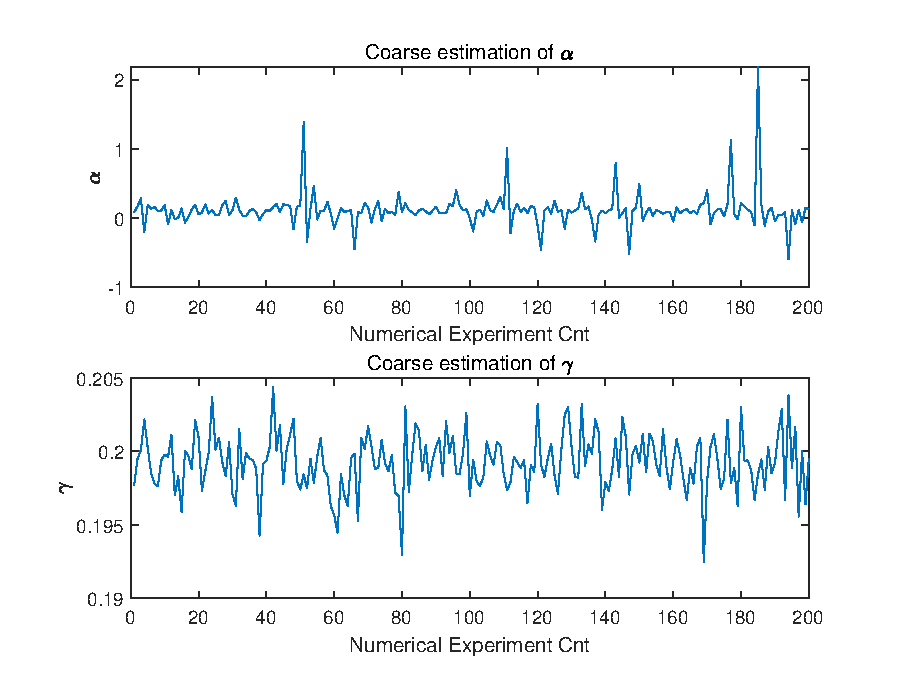
\includegraphics[height=10cm]{../pic/coarse_estimation.eps}
				\caption{Coarse estimation} 
				\label{coarse_ag}
			\end{figure}
			\begin{figure}[!htbp]\centering
				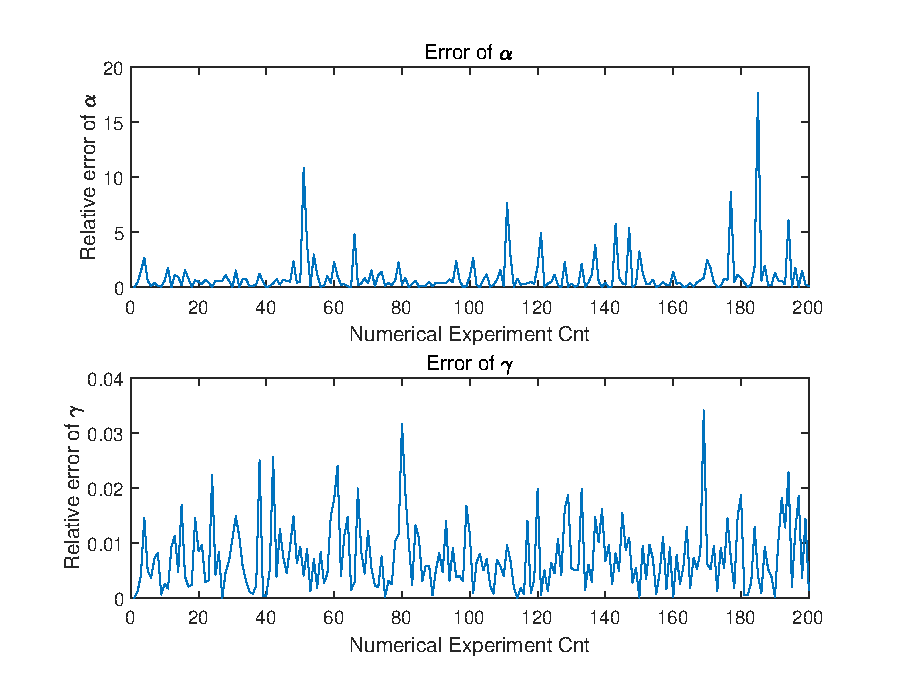
\includegraphics[height=10cm]{../pic/coarse_estimation_err.eps}
				\caption{Error of estimation}
				\label{err_ag}
			\end{figure}
		
			It can be seen from Fig\ref{err_ag} that the error of $\hat{\gamma}$ is about 3\% relative to $\bar{\gamma}$, which is quite nice. But the error of $\hat{\alpha}$ is about 200\% relative to $\bar{\alpha}$, which means that the estimation of $\alpha$ fails in this manner.
			Hence, more sophisticated estimation need to be adopted, although this coarse approach gives relative precise estimation of $\gamma$.\\
			Considering the approach in part(e), where $E(n^2 x)$ is estimated utilizing the info of the noise, similiar approximations can be made as
			\begin{equation}
				E(n^2 x) = E({n^*}^2 x^*) = \frac{\sum_{k=1}^{N}{n_k^*}^2 x_k^*}{N}
			\end{equation}
			and
			\begin{equation}
				E(\dot{n}) = E(\dot{n^*}) = \frac{\sum_{k=2}^{N-1}\dot{n_k^*}}{N-2}
			\end{equation}
			Here, no assumption of the distribution of the noise was made. With $\hat{\gamma}$ given by the coarse estimation, a relative finer estimation of $\hat{\alpha}$ can be calculated as
			\begin{equation}
				\hat{\alpha} = \frac{\hat{\gamma} - E(\dot{n^*})}{E({n^*}^2 x^*)}
			\end{equation} 
			Numerical experiment was carried to verifiy the approximations. This time, the relative error of $\hat{\alpha}$ is satisfying, and the estimation result is
			\begin{equation}
				\begin{aligned}
					\hat{\alpha} & = 0.100805\\
					\hat{\gamma} & = 0.198847
				\end{aligned}
			\end{equation}
			
			Further, we can apply the scheme described in part(e) without tuning  $E(n^2 x)$ finely, just take it as $E({n^*}^2 x^*)$, which also gives similiar result. But these trival stuff will not be discussed here as it has been clear enough for this problem...
	\end{enumerate}

\end{document}